\begin{figure}[t]
    \centering
    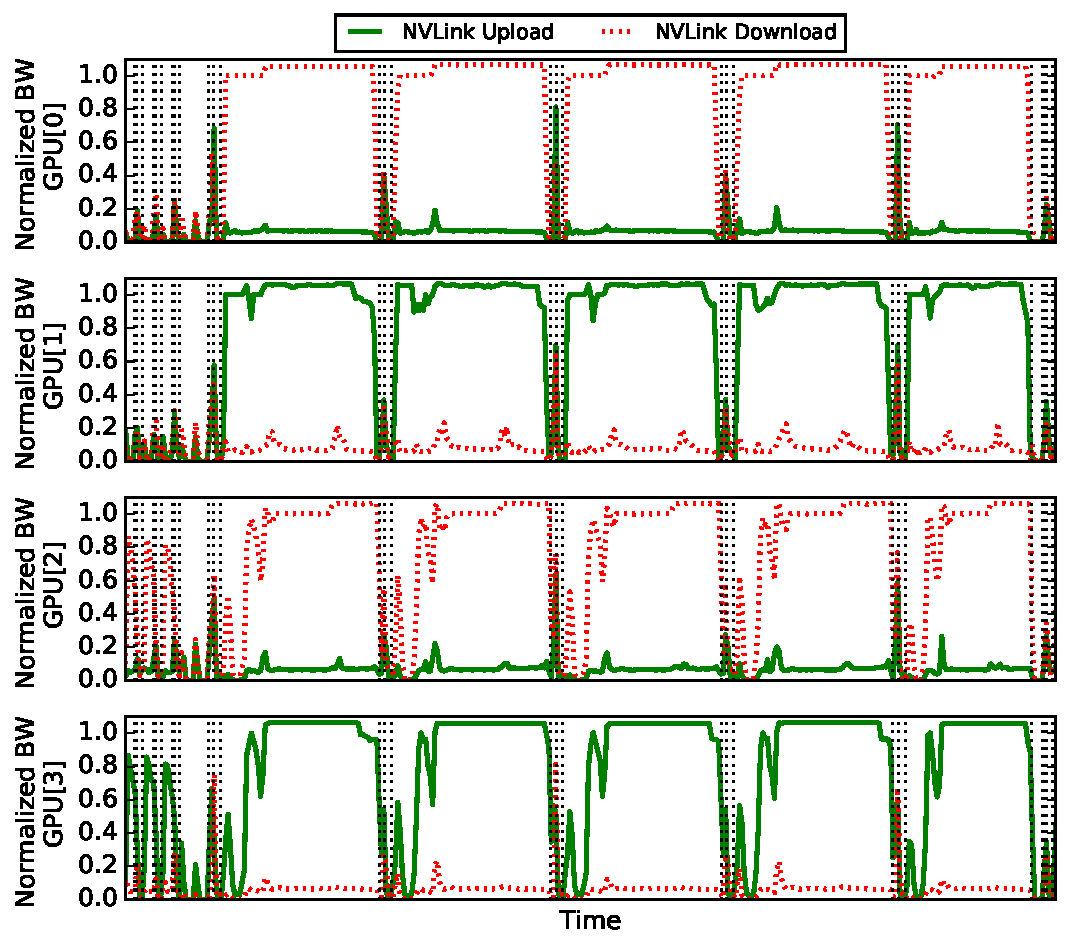
\includegraphics[width=1.0\columnwidth]{figures/bw_profile_HPGMG_UVM_base.pdf}
    \caption{Normalized NVLink bandwidth profile for HPC-HPGMG-UVM showing example of asymmetric 
    link utilization between GPUs and within a GPU depending on kernel and application phasing.}
    \label{fig:link-motivation}
\end{figure}

\section{Asymmetric Interconnects}
\label{interconnect}

The fundamental idea behind asymmetric interconnect management is the following.
In certain applications, executing across a multi-GPU system, 
depending on the current data location, some GPUs have a different utilization 
of the incoming and outgoing interconnect bandwidth. If one of the two directions
is saturated and the other is not, there could be some advantages in trying to 
dynamically reconfigure some of the not saturated links on the direction 
that is saturated.

\begin{figure*}[tp]
    \centering
    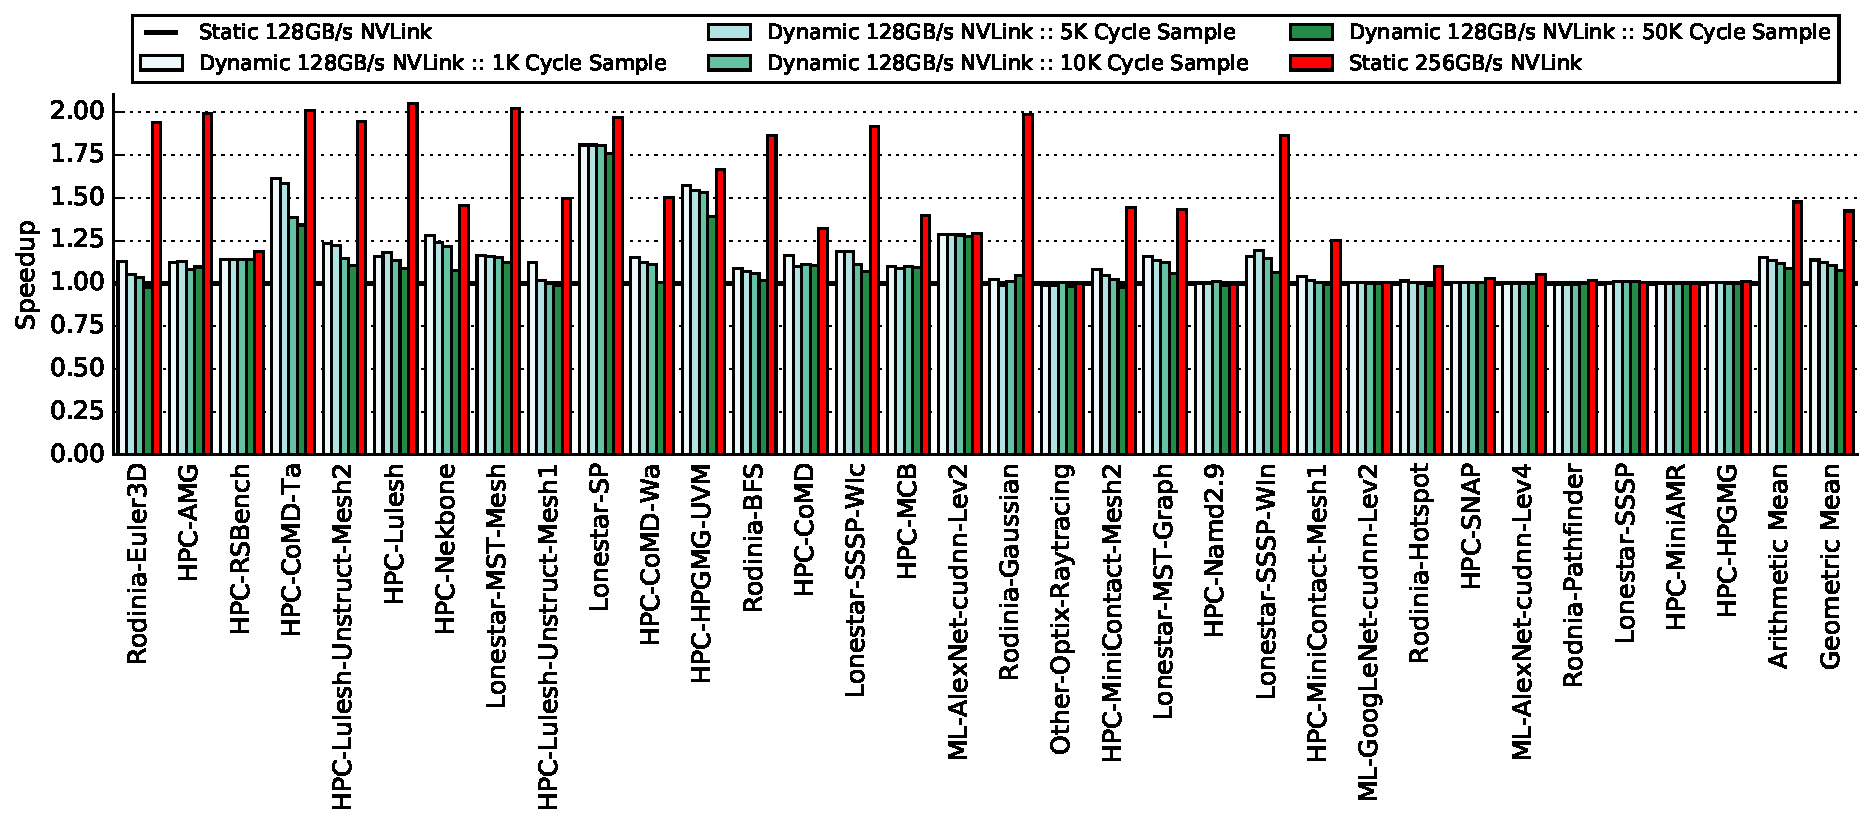
\includegraphics[width=1.0\textwidth]{figures/plot_nvlink_sample_time.pdf}
    \caption{Show that we can adapt to application phasing without too many 
issues}
    \label{fig:sampletime}
\end{figure*}

Figure~\ref{fig:link-motivation} shows the saturation behaviour for a 
snapshot of the UVM optimized HPC-CORAL application 
HPGMG~\cite{adams2014hpgmg} running on our baseline 4 GPUs system. The Figure 
show outgoing and incoming bandwidth utilization for each of the 4 GPUs. 
Vertical dotted black lines represent the beginning kernel calls (which are 
split across the 4 GPUs as explained in Section~\ref{background}). We can see 
that after few initial small kernels (that never reach 1.0 utilization) on any 
of the GPU links, three large kernels start (interleaved by few small 
kernels). On those three large kernels GPU0 and GPU2 fully saturate incoming 
links, while GPU1 and GPU3 fully saturate outgoing links. At the same time 
GPU0 and GPU2 barely use outgoing links and the opposite is true for GPU1 and 
GPU3.

In our simulations we model point-to-point connections composed of multiple 
lanes similarly of those found in NVLink (called Sub-Links in NVidia NVLink 
white-paper~\cite{pascal-tesla-wp}). We use 16 lanes running at 8GB/sec, so 
that each GPU connect to a switch with an aggregate bandwidth of 128GB/sec. 
Our adaptive schemes works as following. By default, whenever a kernel starts 
we begin with 8 lanes per direction (yielding 64GB/sec per direction). 
Periodically we check the saturation status of the lanes. If we find that 
the lanes in one direction are not saturated, while the lanes in the other 
direction are 99\% saturated, we reverse the direction of one of the 
unsaturated lanes. We periodically repeat the check and we stop either when 
equilibrium is reached or all the lanes but one have been reversed (we always 
leave at least a minimum of aggregate 8GB/sec in one direction). If all 
lanes are saturated or not-saturated we do nothing. We have a threshold of 
1GB/sec to prevent switching for minimum variations in traffic shape.

There are two important factors that characterize the above behaviour(i) 
\emph{switch\_time}: the cost of switching the direction a lane (ii) 
\emph{sample\_time}: the frequency at which we want to sample for a possible 
reconfiguration. Since the cost of switching a lane consists in waiting all 
the traffic to be drained from the lane and to physically reconfigure the 
lane to transmit on the other direction, with the term \emph{switch\_time} we 
refer to the later. 



\subsection{Results}
Figure~\ref{fig:sampletime} shows the expected performance improvement, with 
respect to our baseline architecture by exploring different values 
of the ``sample\_time'' and assuming a ``switch\_time'' of 100 cycles 
as reported in \cite{REALLY_NEED_REF_HERE}. Also in Figure~\ref{fig:sampletime}
we show with the \emph{red dash} an upper-bound performance when doubling
the available interconnect to 256GB/sec (128GB/sec per direction). 
We can see that for some applications the dynamic lane switching achieves up to
80\% improvements (``Lonestar-SP''). In average even double the interconnect 
bandwidth we expect to see 50\% improvements while our dynamic solution 
achieves 15\% improvements. We can also see that the sample time plays a 
critical role and a too large sample time doesn't capture application dynamics 
resulting in smaller improvements. We found 5K cycles to be a reasonable sample
time able to achieve good results and never degrade performance. 
In Figure~\ref{fig:switchtime} we used 5K cycles sample time to
explore values of ``switch\_time'' from 10 cycles to 500 cycles.
We found that a faster switch does not produce better results than 100 cycles
but that in few applications a long (500 cycles) switch time results 25\% 
less performance with respect to 100 cycles (``HPC-CORAL-CoMD\_ta'' and 
``HPC-CORAL-CoMD\_wa'').



% Graph 0: We need a stacked-bar graph that shows what’s the percentage of total 
% exe time spent in configs where: both directions are saturated (no room for 
% improvement), only one direction is saturated (here we can improve), none is 
% saturated (we don’t care for this). Do we want to show this as aggregate number 
% of per-GPU?
% We explain the algorithm how and when we increment and decrement the number of 
% sub-channels per direction. Two important parameters: link switch time and 
% sample time.

% Graph 1: baseline is 1x NVLink, upper bound is 2x NVLink, link switch time is 
% 100 cycles, we show the speedup for different sample time values (1K, 2K, 5K, 
% 10K, 100K cycles). Finner measurements are better.

% Graph 2a: baseline is 1x NVLink, upper bound is 2x NVLink, sample\_time is 1K. 
% We swipe through link\_switch\_time (10, 100, 200, 500 cycles). Here, link 
% switch time is important, we want it to be low.

% Graph 2b: the same, but sample\_time is 100K. Here, we do not care about link 
% switch time. The point where it starts to matter is 5K (or 2K) cycles and below. 
% From now on, we assume 100 cycles for link switch time and 5K (or 2K) cycles for 
% sampling period.


% DO NOT REMOVE, we can use this to compute POWER later
%from http://teams.nvidia.com/sites/Corporate/ntech/SiteAssets/downloads/2014/NTECH2014_SlideDecks%20(presented)/7.1_Osborn.pptx
%Power: 8 lanes (TX + RX) at 25GT/s ~= 1.5W
%Area: 8 Lane PHY (8 TX + 8 RX + PLL) ~= 3.3mm^2
%Physical Data: .5pJ/b transferred





\begin{figure*}[tp]
    \centering
    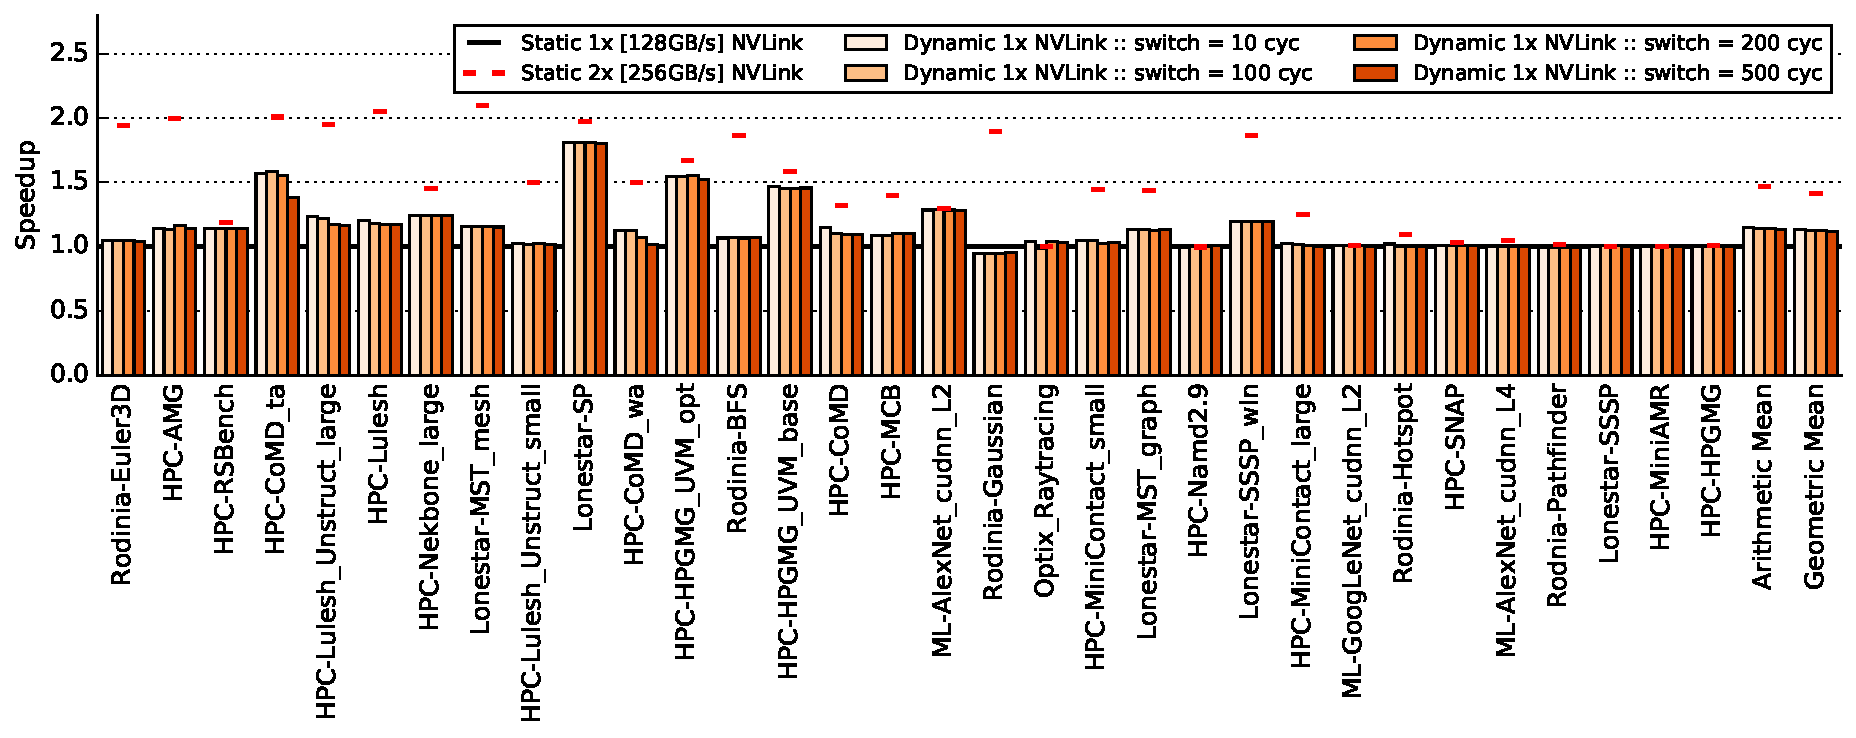
\includegraphics[width=1.0\textwidth]{figures/plot_nvlink_switch_time_sample_time5000.pdf}
    \caption{Show that when we're using a reasonable sample time like even 5k 
cycles, switch time is largely irrelevant, except few 
outliers such as ``HPC-CORAL-CoMD\_ta'' and ``HPC-CORAL-CoMD\_wa''.}
    \label{fig:switchtime}
\end{figure*}